\documentclass[11pt]{article}
\usepackage{listings}
\lstset{
}

\usepackage{fancyhdr}
\pagestyle{fancy}
\newcommand\course{CSC 486B}
\newcommand\hwnumber{3}
\newcommand\duedate{February 8, 2020}

\lhead{Oliver Tonnesen\\V00885732}
\chead{\textbf{\Large Assignment \hwnumber}}
\rhead{\course\\\duedate}

\usepackage{graphicx}

\usepackage{mathtools}
\usepackage{amsmath}


\begin{document}
\abstract{This assignment implements a linear classifier and demonstrates its performance on the CIFAR 10 data set when equipped with different models and features. This report gives a derivation of the gradient for cross entropy loss used in the classifier and a summary of the results obtained, including best classification accuracy and figures generated during training.}


\section*{Derivation of the gradient for cross entropy}
We begin by rewriting $L_i$:
\begin{align*}
	L_i&=-\log\frac{\sum_kt_{ik}e^{s_{ik}}}{\sum_je^{s_{ij}}}\\
	   &=-\log\sum_kt_{ik}p_{ik}\\
	   &=-\sum_k\log t_{ik}p_{ik}
\end{align*}
We find $\frac{\partial L_i}{\partial s_{ik}}$:
\begin{align*}
	\frac{\partial L_i}{\partial s_{ik}}
	&=\frac{\partial(-\sum_k\log t_{ik}p_{ik})}{\partial s_{ik}}\\
	&=-\sum_k\frac{\partial\log t_{ik}p_{ik}}{\partial s_{ik}}\\
	&=-\frac{\partial \log{p_{iy_i}}}{\partial s_{ik}}\\
	&=-\frac{1}{p_{iy_i}}\cdot\frac{\partial p_{iy_i}}{\partial s_{ik}}
\end{align*}
To find $\frac{\partial p_{ij}}{\partial s_{ik}}$, note that it splits into two cases based on whether or not $j=k$.
We first consider the case where $j=k$:
\begin{align*}
	\frac{\partial p_{ij}}{\partial s_{ik}}
	&=\frac{\partial \frac{e^{s_{ij}}}{\sum_l e^{s_{il}}}}{\partial s_{ik}}\\
	&=\frac{e^{s_{ij}}\sum_l e^{s_{ij}}-e^{s_{ij}}e^{s_{ik}}}{\left(\sum_l e^{s_{il}}\right)^2}\\
	&=\frac{e^{s_{ij}}}{\sum_l e^{s_{il}}}\cdot\frac{\sum_l e^{s_{il}}-e^{s_{ik}}}{\sum_l e^{s_{il}}}\\
	&=\frac{e^{s_{ij}}}{\sum_l e^{s_{il}}}\cdot\left(\frac{\sum_l e^{s_{il}}}{\sum_l e^{s_{il}}}-\frac{e^{s_{ik}}}{\sum_l e^{s_{il}}}\right)\\
	&=p_{ij}\left(1-p_{ik}\right)
\end{align*}
Next, we consider the case where $j\neq k$:
\begin{align*}
	\frac{\partial p_{ij}}{\partial s_{ik}}
	&=\frac{\partial \frac{e^{s_{ij}}}{\sum_l e^{s_{il}}}}{\partial s_{ik}}\\
	&=\frac{0-e^{s_{ij}}e^{s_{ik}}}{\left(\sum_l e^{s_{il}}\right)^2}\\
	&=\frac{e^{s_{ij}}}{\sum_l e^{s_{il}}}\cdot\frac{e^{s_{ik}}}{\sum_l e^{s_{il}}}\\
	&=-p_{ij}p_{ik}
\end{align*}
So in the end, we get
\begin{align*}
	\frac{\partial L_i}{\partial s_{ik}}
	&=\begin{cases}
		-\frac{1}{p_{iy_i}}\cdot p_{iy_i}\left(1-p_{ik}\right) & \text{if }y_i=k\\
		-\frac{1}{p_{iy_i}}\cdot\left(-p_{iy_i}p_{ik}\right) & \text{if }y_i\neq k\\
	\end{cases}\\
	&=\begin{cases}
		p_{ik}-1 & \text{if }y_i=k\\
		p_{ik} & \text{if }y_i\neq k\\
	\end{cases}
\end{align*}


\section*{Training curve}
The HOG feature was tested with both the SVM and logistic regression models.
The results can be seen in Figs. \ref{fig:HOG_SVM_Loss}, \ref{fig:HOG_SVM_Acc}, \ref{fig:HOG_Log_Loss}, and \ref{fig:HOG_Log_Acc}.

\begin{figure}[h]
	\begin{minipage}{0.5 \textwidth}
		\centering
		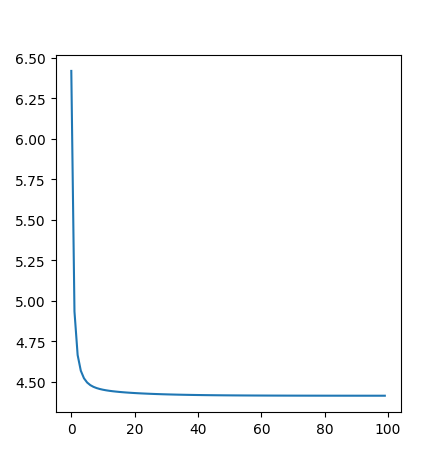
\includegraphics[width=0.8 \textwidth]{figure/HOG_SVM_Loss.png}
		\caption{HOG SVM Loss}
		\label{fig:HOG_SVM_Loss}
	\end{minipage}
	\begin{minipage}{0.5 \textwidth}
		\centering
		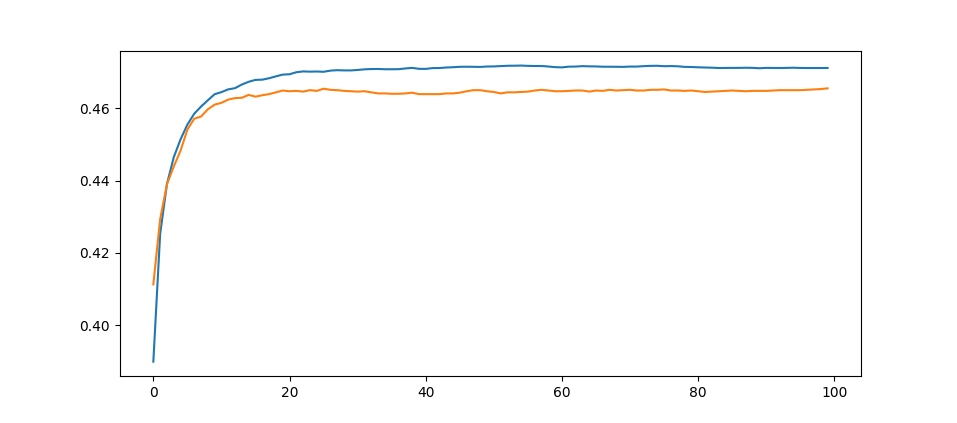
\includegraphics[width=1.4 \textwidth]{figure/HOG_SVM_Acc.png}
		\caption{HOG SVM Accuracy}
		\label{fig:HOG_SVM_Acc}
	\end{minipage}
\end{figure}
\begin{figure}[h]
	\centering
	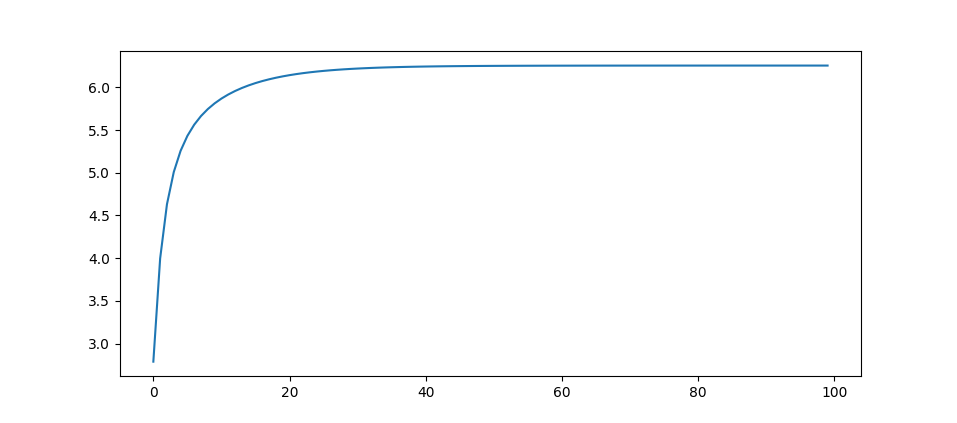
\includegraphics[width=0.5 \textwidth]{figure/HOG_Log_Loss.png}
	\caption{HOG Logistic Regression Loss}
	\label{fig:HOG_Log_Loss}
\end{figure}
\begin{figure}[h]
	\centering
	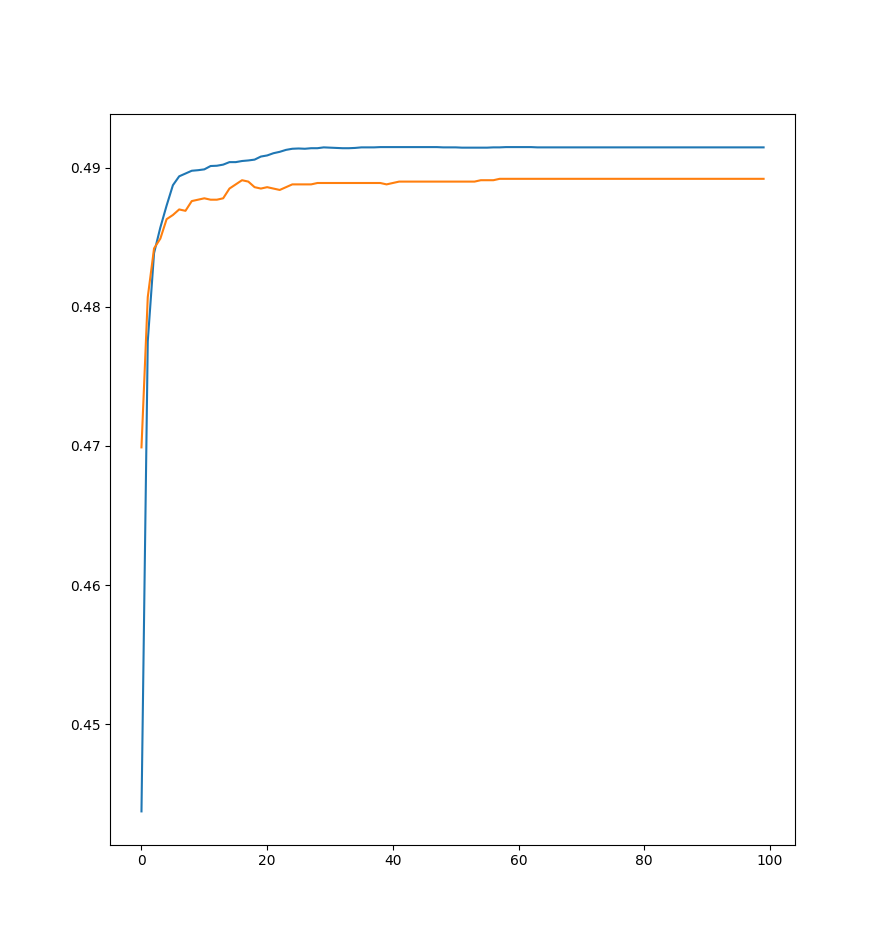
\includegraphics[width=0.5 \textwidth]{figure/HOG_Log_Acc.png}
	\caption{HOG Logistic Regression Accuracy}
	\label{fig:HOG_Log_Acc}
\end{figure}
The model yielding the most highest validation accuracy in conjunction with the HOG feature was logistic regression, with an average validation accuracy of 48.92\%.


\section*{Cross validation results}
We tested the HOG feature with the Logistic Regression model using cross validation with two sets of hyper-parameters: learning rate 0.0001 and reg\_lambda 0.1 resulted in 49.29\% accuracy, and learning rate 0.00012 and reg\_lambda 0.05 resulted in 49.37\% accuracy, the highest achieved.
Below we give the accuracy and loss graphs for these sets of hyper-parameters:
\begin{figure}[h]
	\begin{minipage}{0.5 \textwidth}
		\centering
		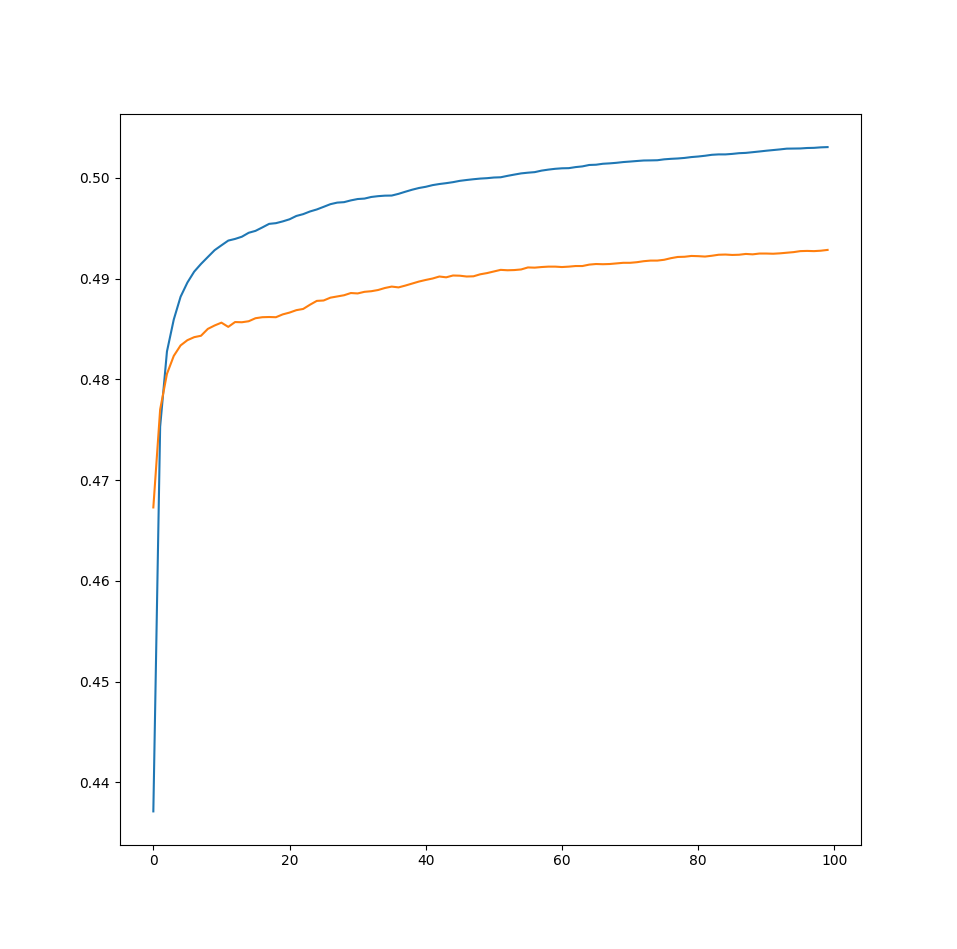
\includegraphics[width=1 \textwidth]{figure/HOG_Log_Acc_Reg-0.1_CV.png}
		\caption{Reg lambda: 0.1, learning rate: 0.0001}
		\label{fig:HOG_Log_Acc_Reg-0.1_CV}
	\end{minipage}
	\begin{minipage}{0.5 \textwidth}
		\centering
		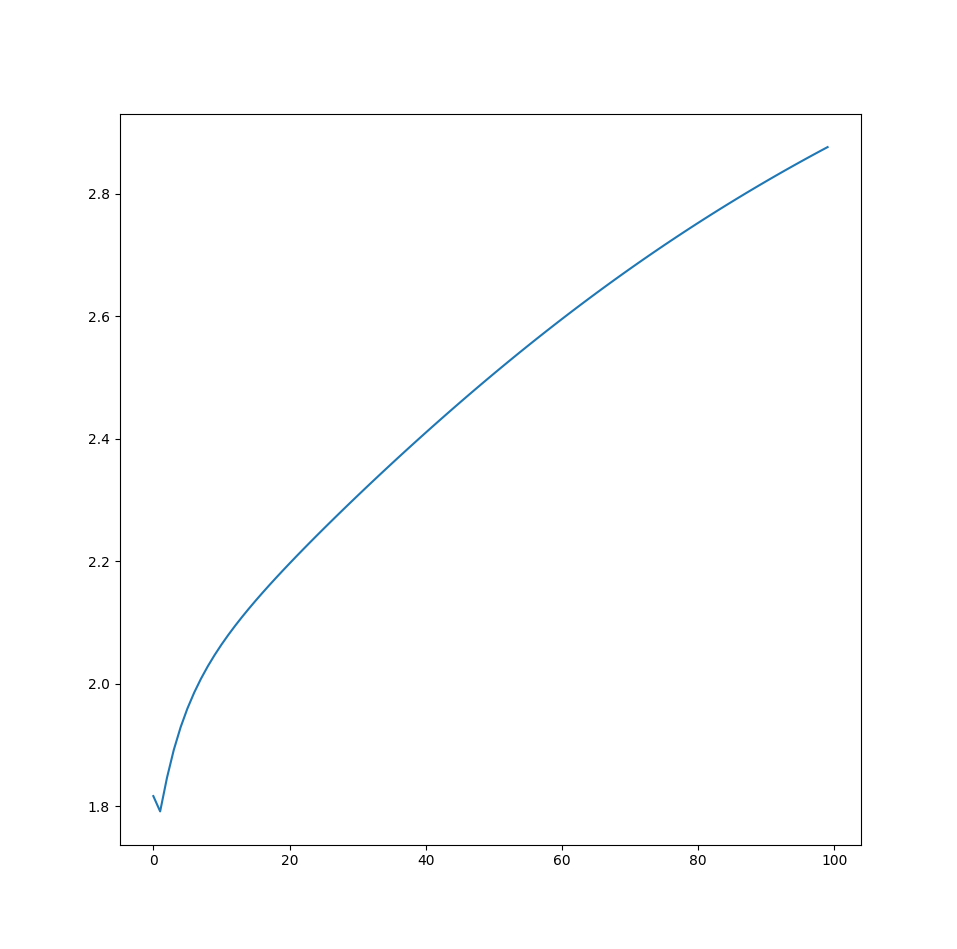
\includegraphics[width=1 \textwidth]{figure/HOG_Log_Loss_Reg-0.1_CV.png}
		\caption{Reg lambda: 0.1, learning rate: 0.0001}
		\label{fig:HOG_Log_Loss_Reg-0.1_CV}
	\end{minipage}
\end{figure}
\begin{figure}[h]
	\begin{minipage}{0.5 \textwidth}
		\centering
		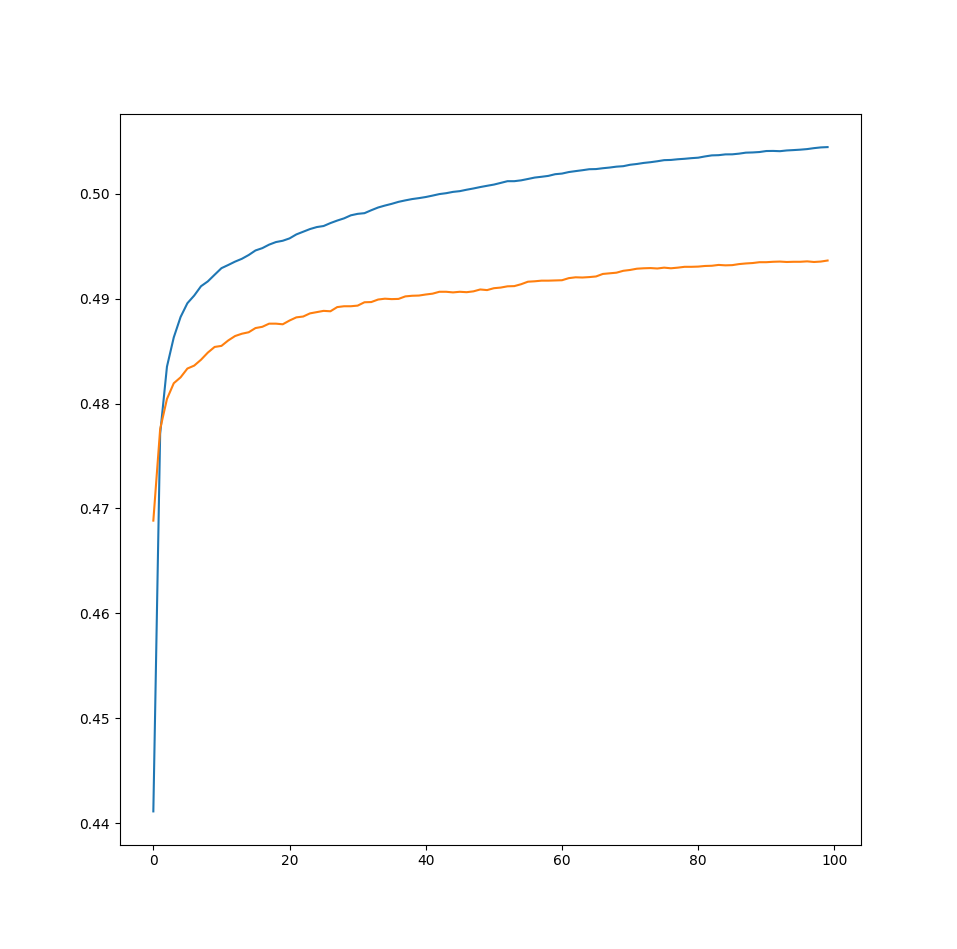
\includegraphics[width=1 \textwidth]{figure/HOG_Log_Acc_Reg-0.05_Learn-0.00012_CV.png}
		\caption{Reg lambda: 0.05, learning rate: 0.00012}
		\label{fig:HOG_Log_Acc_Reg-0.05_Learn-0.00012}
	\end{minipage}
	\begin{minipage}{0.5 \textwidth}
		\centering
		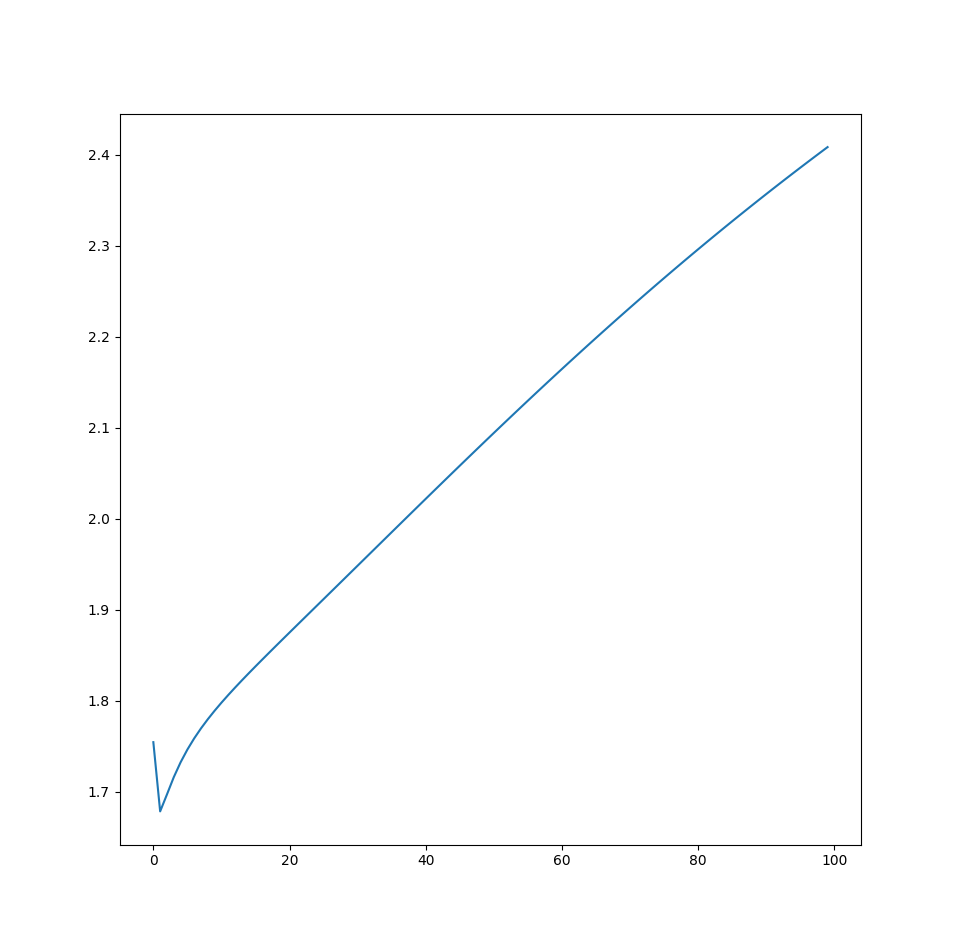
\includegraphics[width=1 \textwidth]{figure/HOG_Log_Loss_Reg-0.05_Learn-0.00012_CV.png}
		\caption{Reg lambda: 0.05, learning rate: 0.00012}
		\label{fig:HOG_Log_Loss_Reg-0.05_Learn-0.00012}
	\end{minipage}
\end{figure}


\end{document}
